\documentclass{article}

\usepackage{graphicx}
\usepackage{tikz}
\usepackage{tikzsymbols}
\usetikzlibrary{calc,patterns,shapes.geometric}
\pagestyle{empty}
\usepackage[margin=0pt]{geometry}
\geometry{papersize={14in,12in}}

\def\centerarc[#1](#2)(#3:#4:#5){\draw[#1] ($(#2)+({#5*cos(#3)},{#5*sin(#3)})$) arc (#3:#4:#5);}

\begin{document}
	\begin{figure}
		\centering
		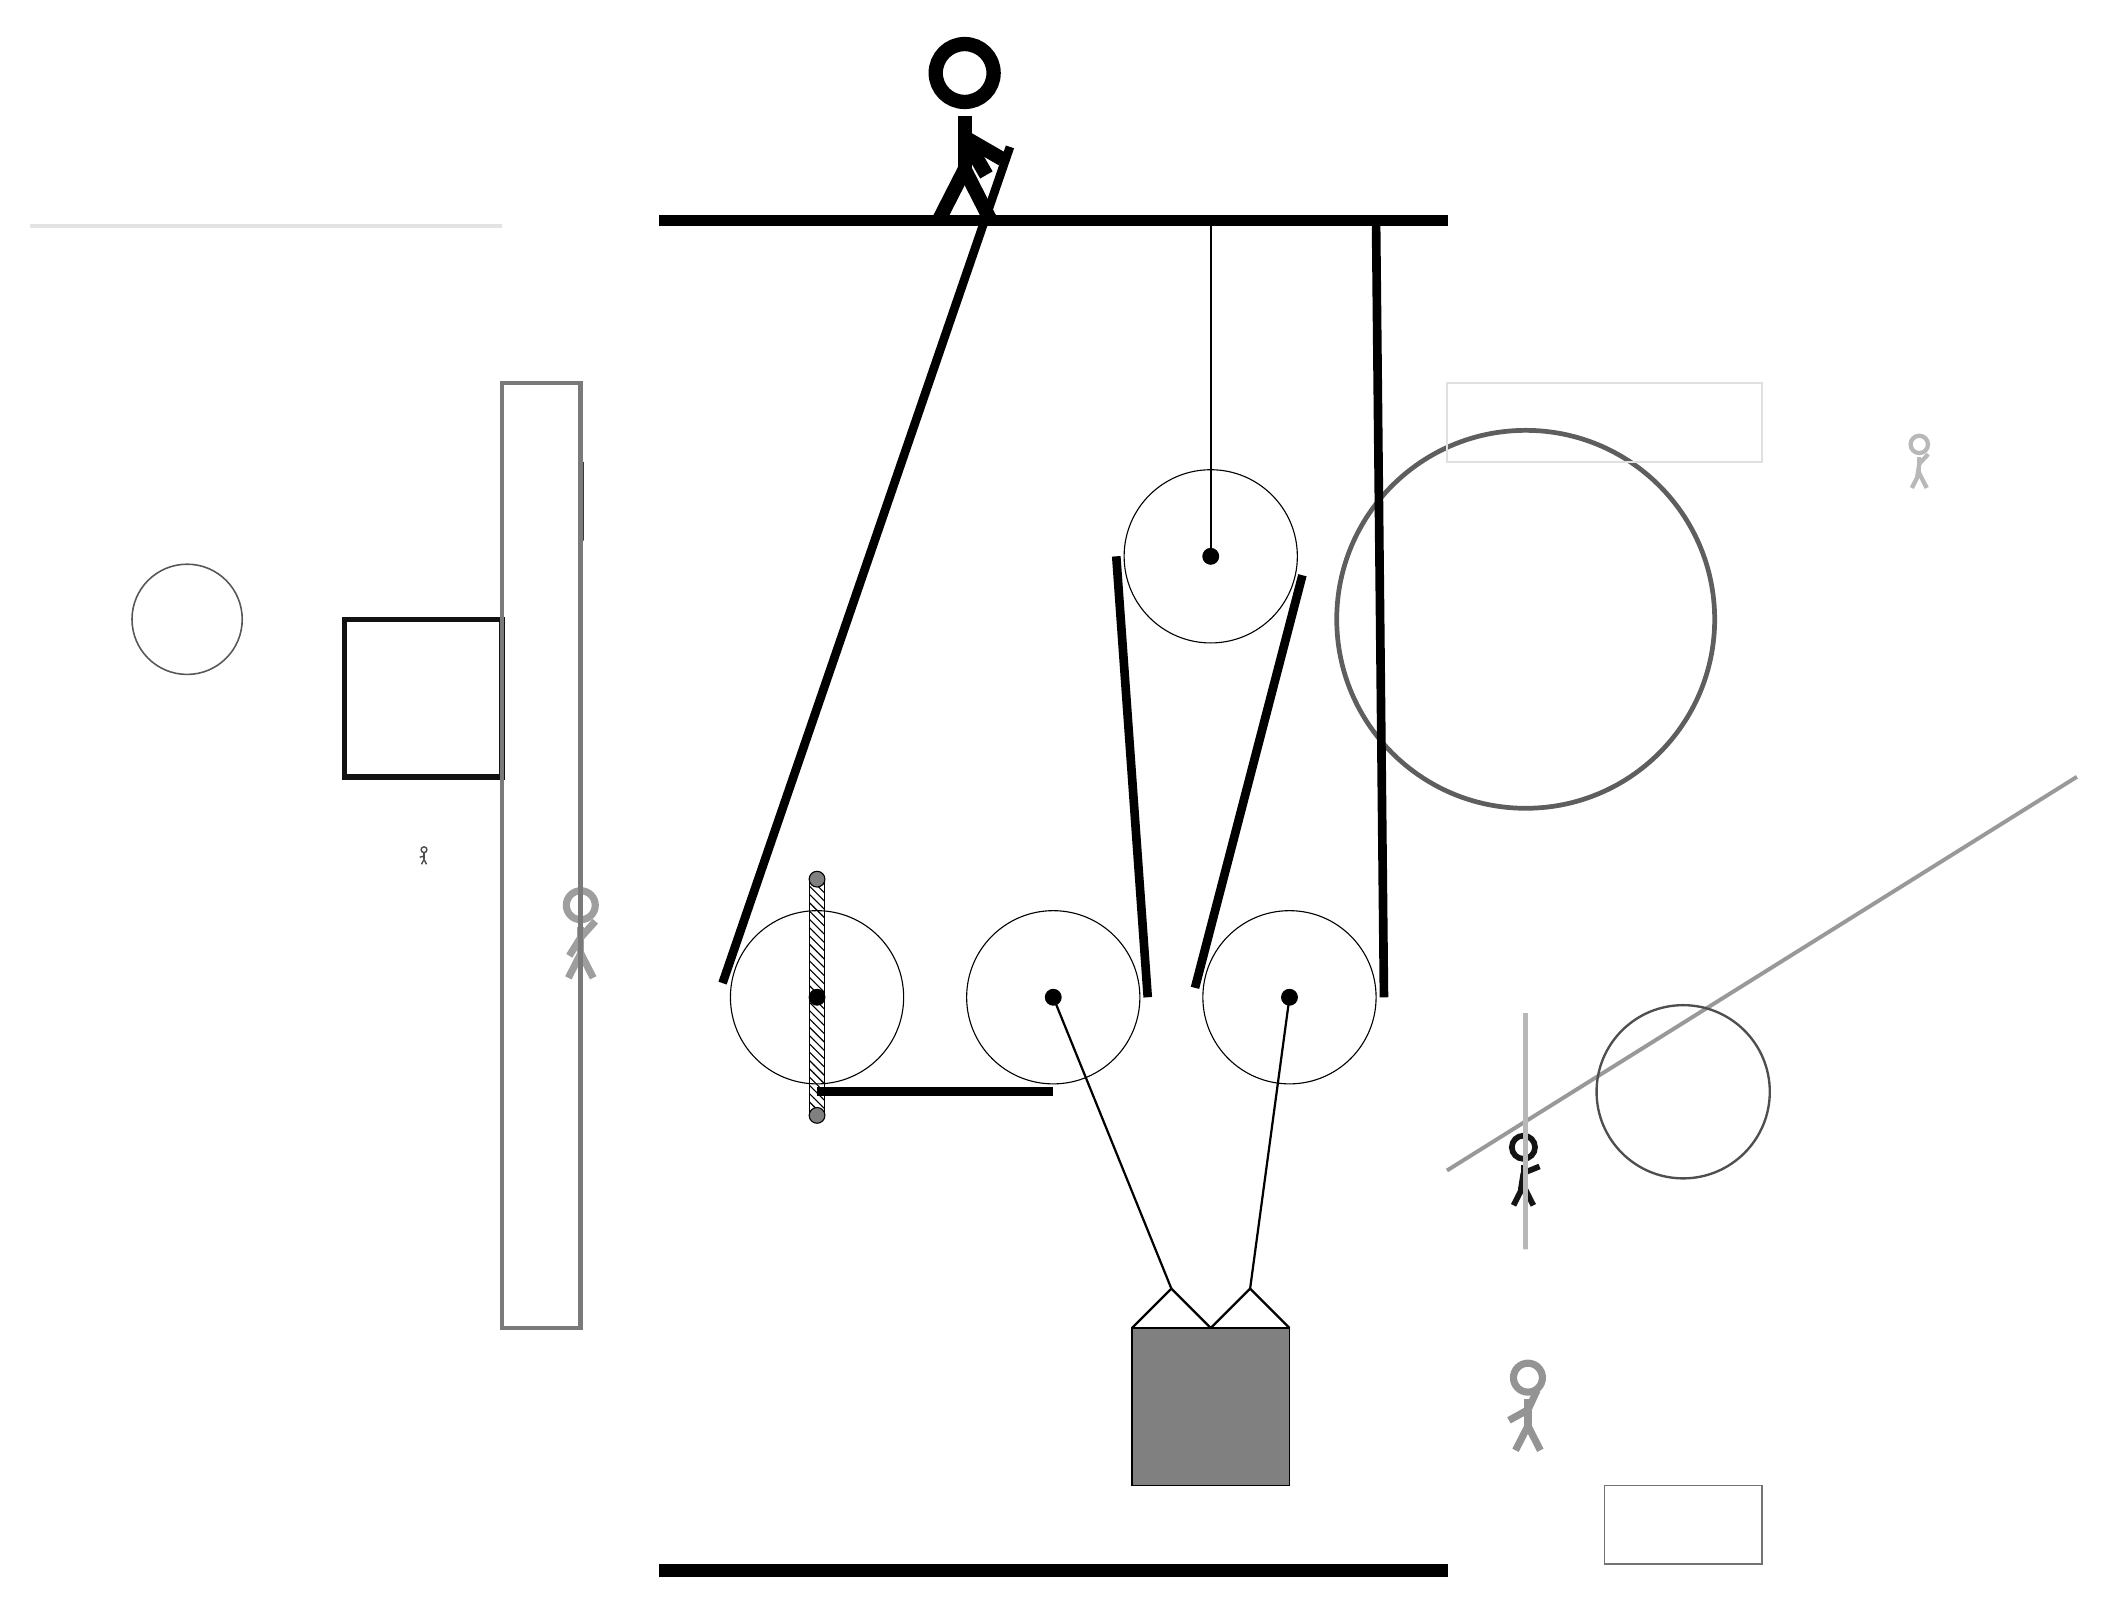
\begin{tikzpicture}
			%%%%% START %%%%%
			
			\draw[fill=black] (-4, 14) rectangle (6, 14.125);
			
			\draw (1, 4.2) circle (1.1);
			\draw[fill=black] (1, 4.2) circle (0.1);
			
			\draw (3, 9.8) circle (1.1);
			\draw[fill=black] (3, 9.8) circle (0.1);
			\draw[thick] (3, 9.8) -- (3, 14);
			
			\draw (4, 4.2) circle (1.1);
			\draw[fill=black] (4, 4.2) circle (0.1);
			
			\draw[line width=0.7mm, color=black!78] (-5, 11) rectangle (-5, 10);
			
			\draw[line width=0.5mm, color=black!40](6, 2) -- (14, 7);
			\node[line width=0.4mm, color=black!92] at (7, 2) {\Strichmaxerl[4][81][22]};
			\draw[line width=0.2mm, color=black!55] (8, -2) rectangle (10, -3);
			
			\node[line width=0.4mm, color=black!42] at (7, -1) {\Strichmaxerl[5][29][65]};
			\draw[line width=0.7mm, color=black!93] (-6, 7) rectangle (-8, 9);
			\node[line width=0.6mm, color=black!70] at (-7, 6) {\Strichmaxerl[1][13][90]};
			\draw [line width=0.6mm, color=black!63](7, 9) circle (2.4);
			\node[line width=0.3mm, color=black!28] at (12, 11) {\Strichmaxerl[3][81][47]};
			\draw[line width=0.6mm, color=black!28] (7, 1) rectangle (7, 4);
			\node[line width=0.7mm, color=black!38] at (-5, 5) {\Strichmaxerl[5][58][48]};
			\draw[line width=0.3mm, color=black!12] (6, 11) rectangle (10, 12);
			\draw[line width=0.6mm, color=black!52] (-5, 12) rectangle (-6, 0);
			
			\draw [line width=0.2mm, color=black!66](-10, 9) circle (0.7);
			\draw[line width=0.5mm, color=black!11](-6, 14) -- (-12, 14);
			\draw [line width=0.3mm, color=black!69](9, 3) circle (1.1);
			
			
			\draw[thick] (4, 4.2) -- (3.5, 0.5);
			\draw[thick] (1, 4.2) -- (2.5, 0.5);
			\draw[thick]  (2, 0) -- (2.5, 0.5) -- (3, 0);
			\draw[thick]  (3, 0) -- (3.5, 0.5) -- (4, 0);
			\draw[fill=black!50] (2, 0) rectangle (4, -2);
			
			\draw (-2, 4.2) circle (1.1);
			\draw[fill=black] (-2, 4.2) circle (0.1);
			\draw[pattern=north west lines, pattern color=black] (-2.1, 5.7) rectangle (-1.9, 2.7);
			\draw[fill=black!50] (-2, 5.7) circle (0.1);
			\draw[fill=black!50] (-2, 2.7) circle (0.1);
			
			\draw[line width=1.1mm] (0.45, 15) -- (-3.2, 4.38);
			\centerarc[line width=1.1mm](-2, 4.2)(160:270:1.2000000000000002);
			\draw[line width=1.1mm](-2, 3.0) -- (1, 3.0);
			\centerarc[line width=1.1mm](1, 4.2)(270:360:1.2000000000000002);
			\draw[line width=1.1mm] (2.2, 4.2) -- (1.8, 9.8);
			\centerarc[line width=1.1mm](3, 9.8)(-20:180:1.2000000000000002);
			\draw[line width=1.1mm](4.164, 9.56) -- (2.8, 4.32);
			\centerarc[line width=1.1mm](4, 4.2)(160:360:1.2000000000000002);
			\draw[line width=1.1mm](5.2, 4.2) -- (5.1, 14);
			
			\node at (-0.07, 15.2) {\Strichmaxerl[10][120][-30]};
			
			\draw[fill=black] (-4, -3) rectangle (6, -3.15);
			
			%%%%% END %%%%%
		\end{tikzpicture}
	\end{figure}	
\end{document}